\begin{figure}[H]
  \centering
  \pgfplotsset{
  	    scaled y ticks=false,
    scale only axis,
    legend style={at={(0,0.8)}, anchor=west  , font=\tiny
    },
    xmin=7,
  }
  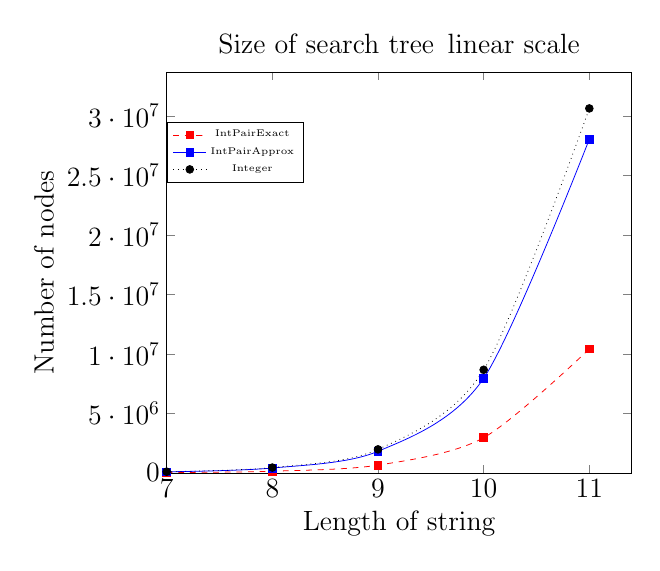
\begin{tikzpicture} [scale=0.7, font=\Large]
    \begin{axis}[
        title=Size of search tree\, linear scale,
        ylabel=Number of nodes,
        xtick=data,
        ymin=0, 
        xlabel=Length of string]
      \addplot[smooth,mark=square*, mark options={solid},red, dashed]
      coordinates{ (7,33465) (8,146201) (9,658312) (10,2959824) (11,10414734)
      }; %\label{ie_plot}
      \addlegendentry{IntPairExact}
      \addplot[smooth,mark=square*, mark options={solid},blue]
      coordinates{ (7,97813) (8,414505) (9,1819264) (10,7950138) (11,28032604)
      }; %\label{ia_plot}
      \addlegendentry{IntPairApprox}
      \addplot[smooth,mark=*,mark options={solid},black, dotted]
      coordinates{ (7,107122) (8,453696) (9,1981650) (10,8664862) (11,30614378)
      }; %\label{int_plot}
      \addlegendentry{Integer}
    \end{axis}
  \end{tikzpicture}
  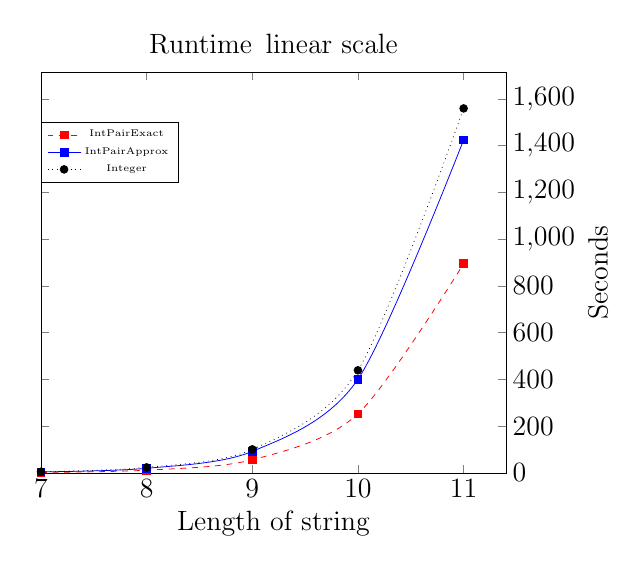
\begin{tikzpicture} [scale=0.7, font=\Large]
    \begin{axis}[
        yticklabel pos=right,
        xtick=data,
        title=Runtime\, linear scale,
        ylabel=Seconds,
        xlabel=Length of string,
        ymin=0, ]
      \addplot[smooth,mark=square*,mark options={solid},red, dashed]
      coordinates{ (7, 2.256) (8, 11.920) (9, 56.407) (10, 252.762) (11, 894.726)
      };% \label{IntPairExact Run}
      \addplot[smooth,mark=square*,mark options={solid},blue]
      coordinates{ (7, 4.721) (8, 19.793) (9, 92.335) (10, 400.819) (11, 1424.025)
      }; %\label{IntPairApprox Run}
      \addplot[smooth,mark=*,mark options={solid},black, dotted]
      coordinates{ (7, 5.248) (8, 23.749) (9, 100.874) (10, 438.791) (11, 1558.550)
      }; %\label{IntegerRun}
      \addlegendentry{IntPairExact}
      \addlegendentry{IntPairApprox}
      \addlegendentry{Integer}
    \end{axis}
  \end{tikzpicture}

  
\begin{tikzpicture}[scale=1.4]
    \draw[very thick] (-4,0) -- (4,0);
    \draw[draw=white] (-5,-0.2) -- (5,-0.2);
  \end{tikzpicture}


  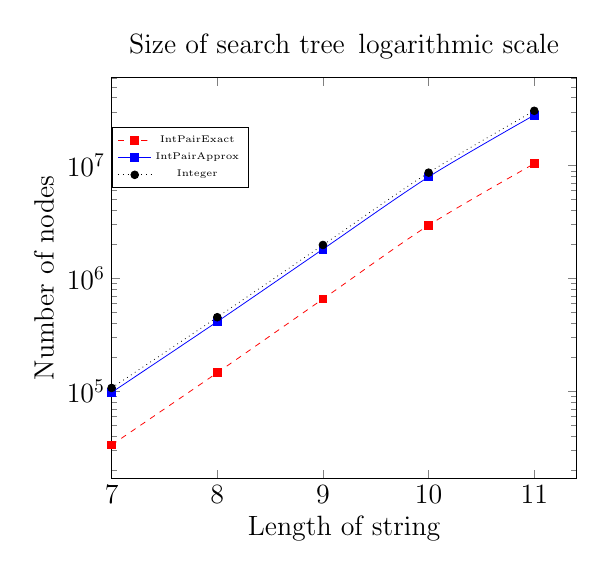
\begin{tikzpicture} [scale=0.7, font=\Large]
    \begin{semilogyaxis}[
        title=Size of search tree\, logarithmic scale,
        ylabel=Number of nodes,
        xtick=data,
        ymin=0, 
        xlabel=Length of string ]
     \addplot[smooth,mark=square*, mark options={solid},red, dashed]
      coordinates{ (7,33465) (8,146201) (9,658312) (10,2959824) (11,10414734)
      }; %\label{ie_plot}
      \addlegendentry{IntPairExact}
      \addplot[smooth,mark=square*, mark options={solid},blue]
      coordinates{ (7,97813) (8,414505) (9,1819264) (10,7950138) (11,28032604)
      }; %\label{ia_plot}
      \addlegendentry{IntPairApprox}
      \addplot[smooth,mark=*,mark options={solid},black, dotted]
      coordinates{ (7,107122) (8,453696) (9,1981650) (10,8664862) (11,30614378)
      }; %\label{int_plot}
      \addlegendentry{Integer}

    \end{semilogyaxis}
  \end{tikzpicture}
  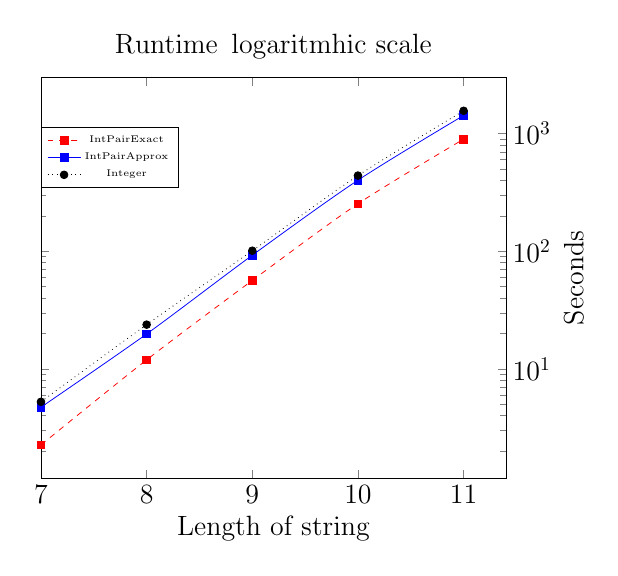
\begin{tikzpicture} [scale=0.7, font=\Large]
    \begin{semilogyaxis}[
        title=Runtime\, logaritmhic scale,
        yticklabel pos=right,
        xtick=data,
        ylabel=Seconds,
        xlabel=Length of string,
        ymin=0,  ]
      \addplot[smooth,mark=square*,mark options={solid},red, dashed]
      coordinates{ (7, 2.256) (8, 11.920) (9, 56.407) (10, 252.762) (11, 894.726)
      };% \label{IntPairExact Run}
      \addplot[smooth,mark=square*,mark options={solid},blue]
      coordinates{ (7, 4.721) (8, 19.793) (9, 92.335) (10, 400.819) (11, 1424.025)
      }; %\label{IntPairApprox Run}
      \addplot[smooth,mark=*,mark options={solid},black, dotted]
      coordinates{ (7, 5.248) (8, 23.749) (9, 100.874) (10, 438.791) (11, 1558.550)
      }; %\label{IntegerRun}
      \addlegendentry{IntPairExact}
      \addlegendentry{IntPairApprox}
      \addlegendentry{Integer}
    \end{semilogyaxis}
  \end{tikzpicture}
  \caption{Varying the length of the string. The other parameters are fixed. Number of states=7, size of alphabet=7, and max cost per transition=15. Here we also show graphs in logarithmic scale.}\label{fig:steps}
\end{figure}
